\documentclass[a4paper]{article}


\usepackage[
    style=numeric, 
    backend=biber, 
    sorting=none
]{biblatex}
\usepackage{graphicx}
\usepackage{enumitem}
\usepackage{geometry}
\usepackage{sectsty}
\usepackage{indentfirst}
\usepackage{times}

\setlist{
  listparindent=\parindent,
  parsep=0pt,
}

\sectionfont{\centering}
\addbibresource{citation.bib}
\graphicspath{{./images/}}
\geometry{a4paper, top=4.0cm, bottom=3.0cm,
          left=4.0cm, includehead, includefoot}
\renewcommand\contentsname{Daftar Pustaka}
\emergencystretch=2em

\begin{document}
\linespread{1.5}

\title{Marketplace For Hobby}
\author{Aldih Suhandi, Chandra Wijaya, Ibrahim Seto Aditama}

\maketitle
\begin{figure}[h]
    \centering
    
\includegraphics[width=10cm]{logo_binus.png}\\
    Binus University\\
    2022
\end{figure}
\begin{figure}[h]
    \centering
    Diperiksa Oleh**\\
    \vspace{15mm}
    \begin{tabular}{@{}p{2.5in}@{}}
    \centering
    Nama Dosen - Kode Dosen
    \end{tabular}
\end{figure}

\newpage
\addcontentsline{toc}{section}{\protect\numberline{}Daftar Pustaka}
\tableofcontents

\newpage
\section*{Pendahuluan}
\addcontentsline{toc}{section}{\protect\numberline{}Pendahuluan}

\newpage
\section*{Tinjauan Pustaka}
\addcontentsline{toc}{section}{\protect\numberline{}Tinjauan Pustaka}
% OOP, Functional Programming, Design Pattern, Architecural Pattern

\begin{enumerate}
    \item \textit{Object Oriented Programming}

    \textit{Object Oriented Programming} adalah konsep programming yang berdasarkan \textit{objects}, sebuah \textit{object} adalah sesuatu entitas yang ada didunia nyata yang bisa diindetifikasi secara unik\autocite{liang_liang_2021}. Sebagai contoh, sebuah meja, seorang guru, dan bahkan hutang bisa dijadikan sebagai \textit{object}. 

    Untuk membuat sebuah \textit{object} diperlukan sebuah \textit{template} atau \textit{blueprint}, \textit{template} atau \textit{blueprint} ini dalam \textbf{OOP} disebut sebagai \textit{class}, secara definisi \textit{class} adalah sebuah \textit{blueprint} yang dipakai untuk membuat sesuatu atau \textit{object} yang lebih spesifik atau konkrit\autocite{education-erin-oop-2020}, \textit{class} biasanya hanya menampung atribut - atribut yang secara general, seperti tinggi, berat badan, umur, dan sebagainya. Sedangkan sebuah \textit{object} akan menampung \textit{value} yang lebih spesifik, seperti \textit{object} tersebut bertinggi 2 meter dan \textit{object} sudah berumur 3 tahun.

    \textbf{OOP} memiliki 4 pilar pendukung, yaitu:
    \begin{itemize}
        \item \textit{Inheritance}

        \textit{Inheritance} adalah sebuah konsep dimana \textit{class} dapat mempunyai atribut dan fitur turunan dari \textit{class} lain. \textit{Class} yang mendapat fitur turunan ini disebut \textit{child class}, sedangkan \textit{class} yang diturunkan disebut \textit{parent class}\autocite{education-erin-oop-2020}. 

        Tujuan dari konsep ini adalah untuk mengurangi redudansi sebanyak mungkin, dengan cara mengeneralisasikan beberapa \textit{class}, karena beberapa \textit{class} yang berbeda bisa saya memiliki fitur atau atribute yang sama. Sebagai contoh \textit{class} guru, murid, dan kepala sekolah memiliki beberapa atribut yang sama, seperti tinggi badan, berat badan, dan umur. Semua atribut yang sama tersebut bisa dijadikan sebuah \textit{parent class} yang bernama \textit{human} dan \textit{class} guru, murid, dan kepala sekolah akan menjadi \textit{child class} dari \textit{class} tersebut\autocite{liang_liang_2021}.

        \begin{figure}
            \centering
            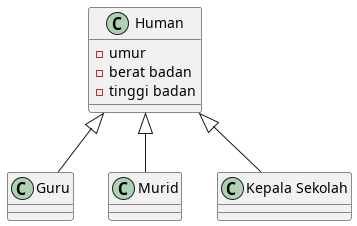
\includegraphics[width=8cm]{inheritance example.png}
            \caption{Contoh dari \textit{inheritance}}
        \end{figure}


        \item \textit{Encapsulation}
        \item \textit{Abstraction}
        \item \textit{Polymorphism}
    \end{itemize}

\end{enumerate}

\newpage
\section*{Metode Pelaksanaan}
\addcontentsline{toc}{section}{\protect\numberline{}Metode Pelaksanaan}

\subsection*{\textit{Tech Stack}}
\addcontentsline{toc}{subsection}{\protect\numberline{}\textit{Tech Stack}}
% mysql
% springboot
% reactjs base framework
% payment API TODO: aldih

\subsection*{System Architecture}
\addcontentsline{toc}{subsection}{\protect\numberline{}System Architecture}
% usecase diagram
% activity diagram
% sequence diagram secara general
% mock up aplikasi

\subsection*{Aplikasi Serupa}
\addcontentsline{toc}{subsection}{\protect\numberline{}Aplikasi Serupa}
% bikin table
% buat +- dari aplikasi serupa ini

\subsection*{Pengumpulan Data Pengguna}
\addcontentsline{toc}{subsection}{\protect\numberline{}Pengumpulan Data Pengguna}

\newpage
\addcontentsline{toc}{section}{\protect\numberline{}Referensi}
\printbibliography[title=Referensi]

\end{document}
